\documentclass[12pt, a4paper, oneside, UTF8]{ctexart}
\usepackage{hyperref}
\usepackage{graphicx}

\begin{document}
已知 Sellmeier 公式为
\begin{equation}
n^{2} = 1 + \sum_{j=1}^{m}\frac{A_{j}\lambda _{j}^{2}}{\lambda^{2}-\lambda _{j}^{2} }
\end{equation}

现在取三阶,即

\begin{equation}
    n^{2}(\lambda) = 1 + \frac{B_1 \lambda^2}{\lambda^2 - C_1^2} + \frac{B_2 \lambda^2}{\lambda^2 - C_2^2}
+ \frac{B_3 \lambda^2}{\lambda^2 - C_3^2}
\end{equation}\\
所以,在拟合的过程中,需要将$B_1,C_1$ 等 6 个参数待定。

\href{https://refractiveindex.info/?shelf=main&book=SiO2&page=Malitson}{网页}上给出的色散公式为
\begin{equation}
    n^{2}(\lambda) = 1 + \frac{0.6961663 \lambda^2}{\lambda^2 - 0.0684043^2} + \frac{0.4079426 \lambda^2}{\lambda^2 - 0.1162414^2}
+ \frac{0.8974794 \lambda^2}{\lambda^2 - 9.896161^2}
\end{equation}
\\

整个过程如下:

①获取波长 \@$\lambda$\@ 和折射率 \@$n$\@ 的数据。本文通过网络爬虫,将\href{https://refractiveindex.info/?shelf=main&book=SiO2&page=Malitson}{网页}上的 \@$101$\@ 组数据保存下来,
具体数据可以查看 \@data.txt\@ 文件;

②确定所要拟合函数的表达式,本文取式(2);

③使用 \@python\@ 第三方库 \@scipy\@ 进行非线性拟合。
\\

按照式(3),波长和折射率的曲线如图\@ 1所示。按照式(2),并给 6 个参数设置取值范围,拟合后波长和折射率的曲线如图\@ 2所示。为了能够有对照组,同样按照式(2),但不给其参数设置取值范围,
得到拟合后的曲线如图\@ 3所示。原始的\@ Sellmeir \@公式以及将参数取值范围限制后拟合的曲线对比,如图\@ 4所示。

因此,最终拟合后的式子为:
\begin{equation}
    n^{2}(\lambda) = 1 + \frac{0.6999999 \lambda^2}{\lambda^2 - 0.0699999^2} + \frac{0.4099999 \lambda^2}{\lambda^2 - 0.1857398^2}
+ \frac{0.8 \lambda^2}{\lambda^2 - 9.999999^2}
\end{equation}

\begin{figure}[htbp]
    \centering
    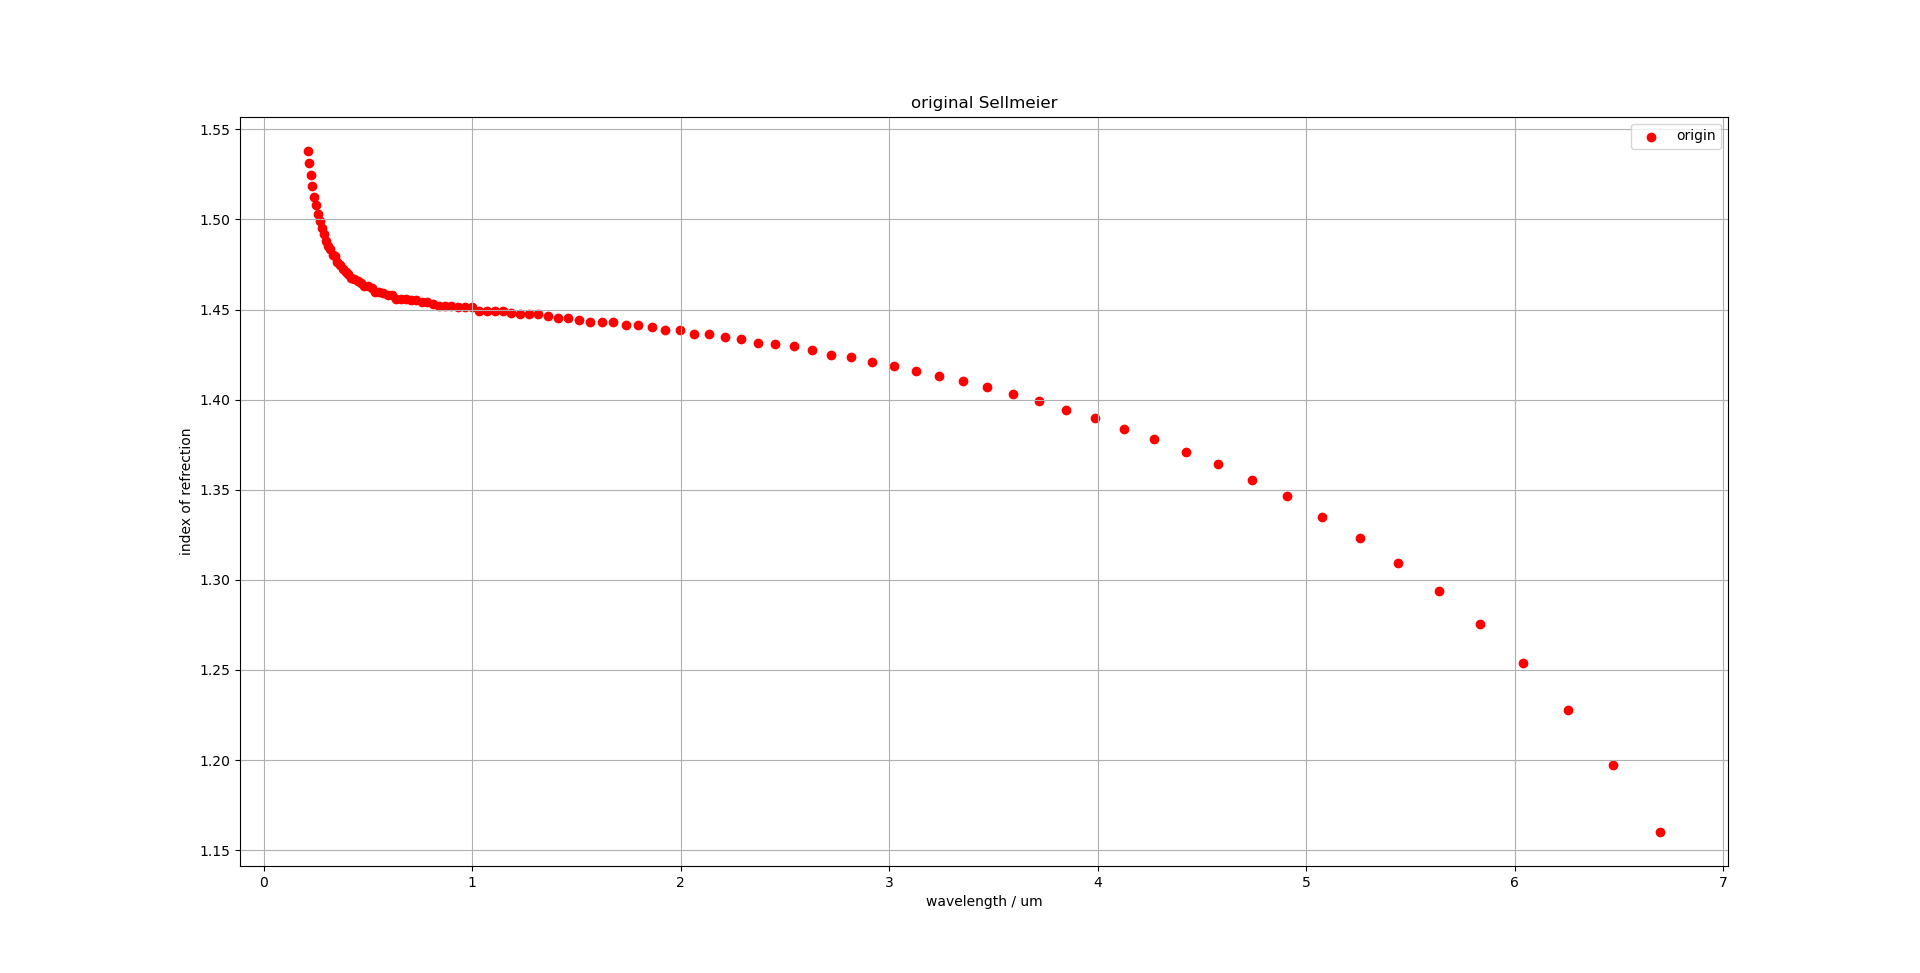
\includegraphics[width=.81\textwidth]{origin.png}
    \caption{原始Sellmeir公式曲线}
\end{figure}
\begin{figure}[htbp]
    \centering
    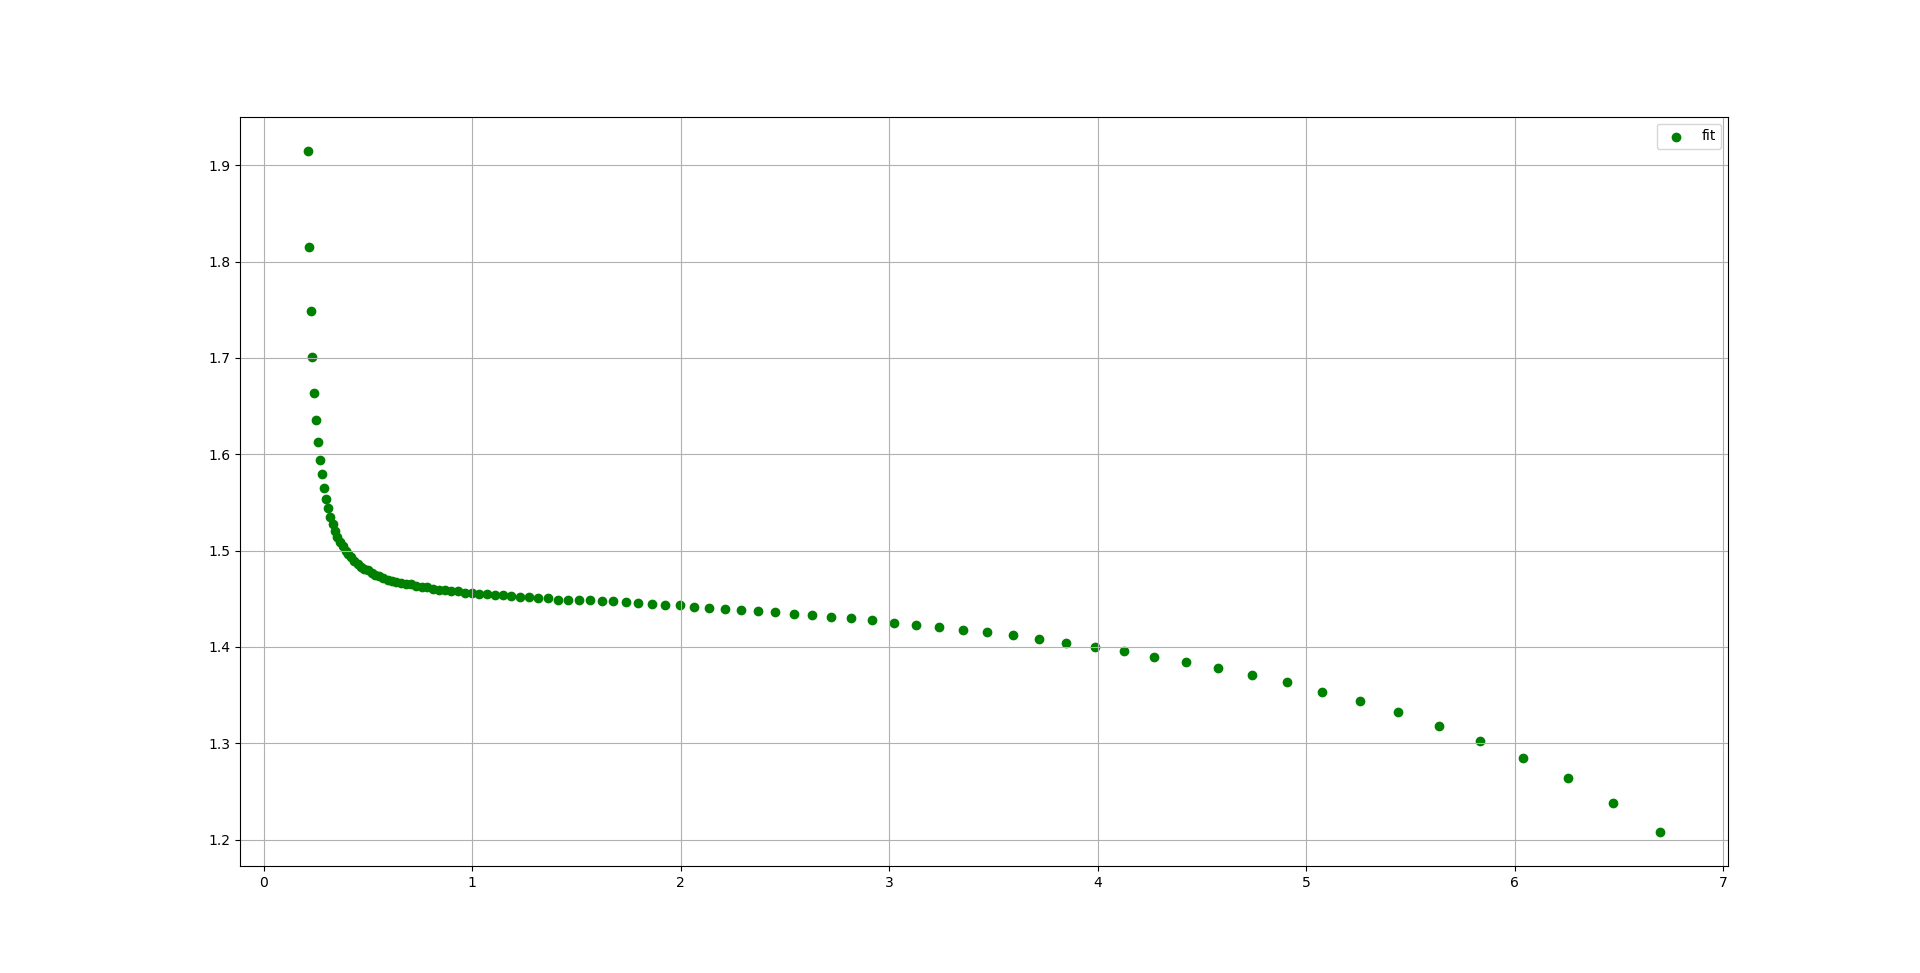
\includegraphics[width=.81\textwidth]{fit.png}
    \caption{参数限制取值范围拟合后Sellmeir公式曲线}
\end{figure}
\begin{figure}[htbp]
    \centering
    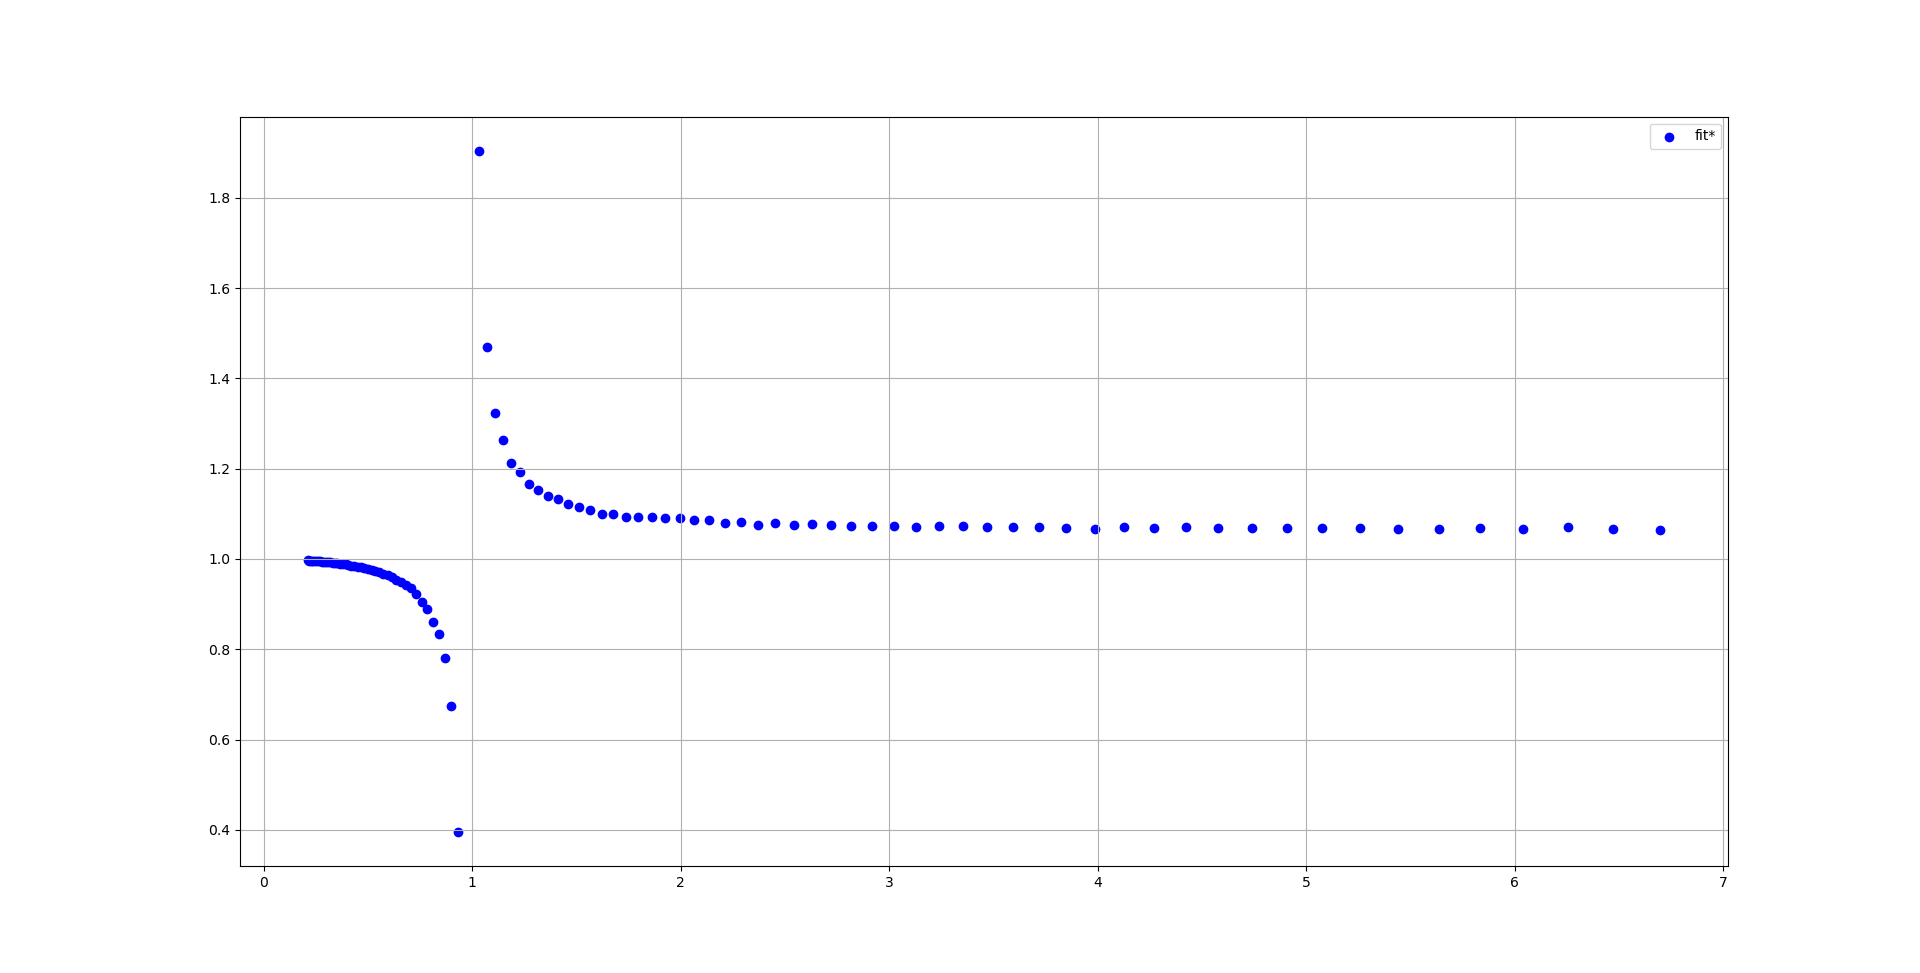
\includegraphics[width=.81\textwidth]{fitnew.png}
    \caption{参数取值无限制拟合后Sellmeir公式曲线}
\end{figure}

\newpage
\begin{figure}[htbp]
    \centering
    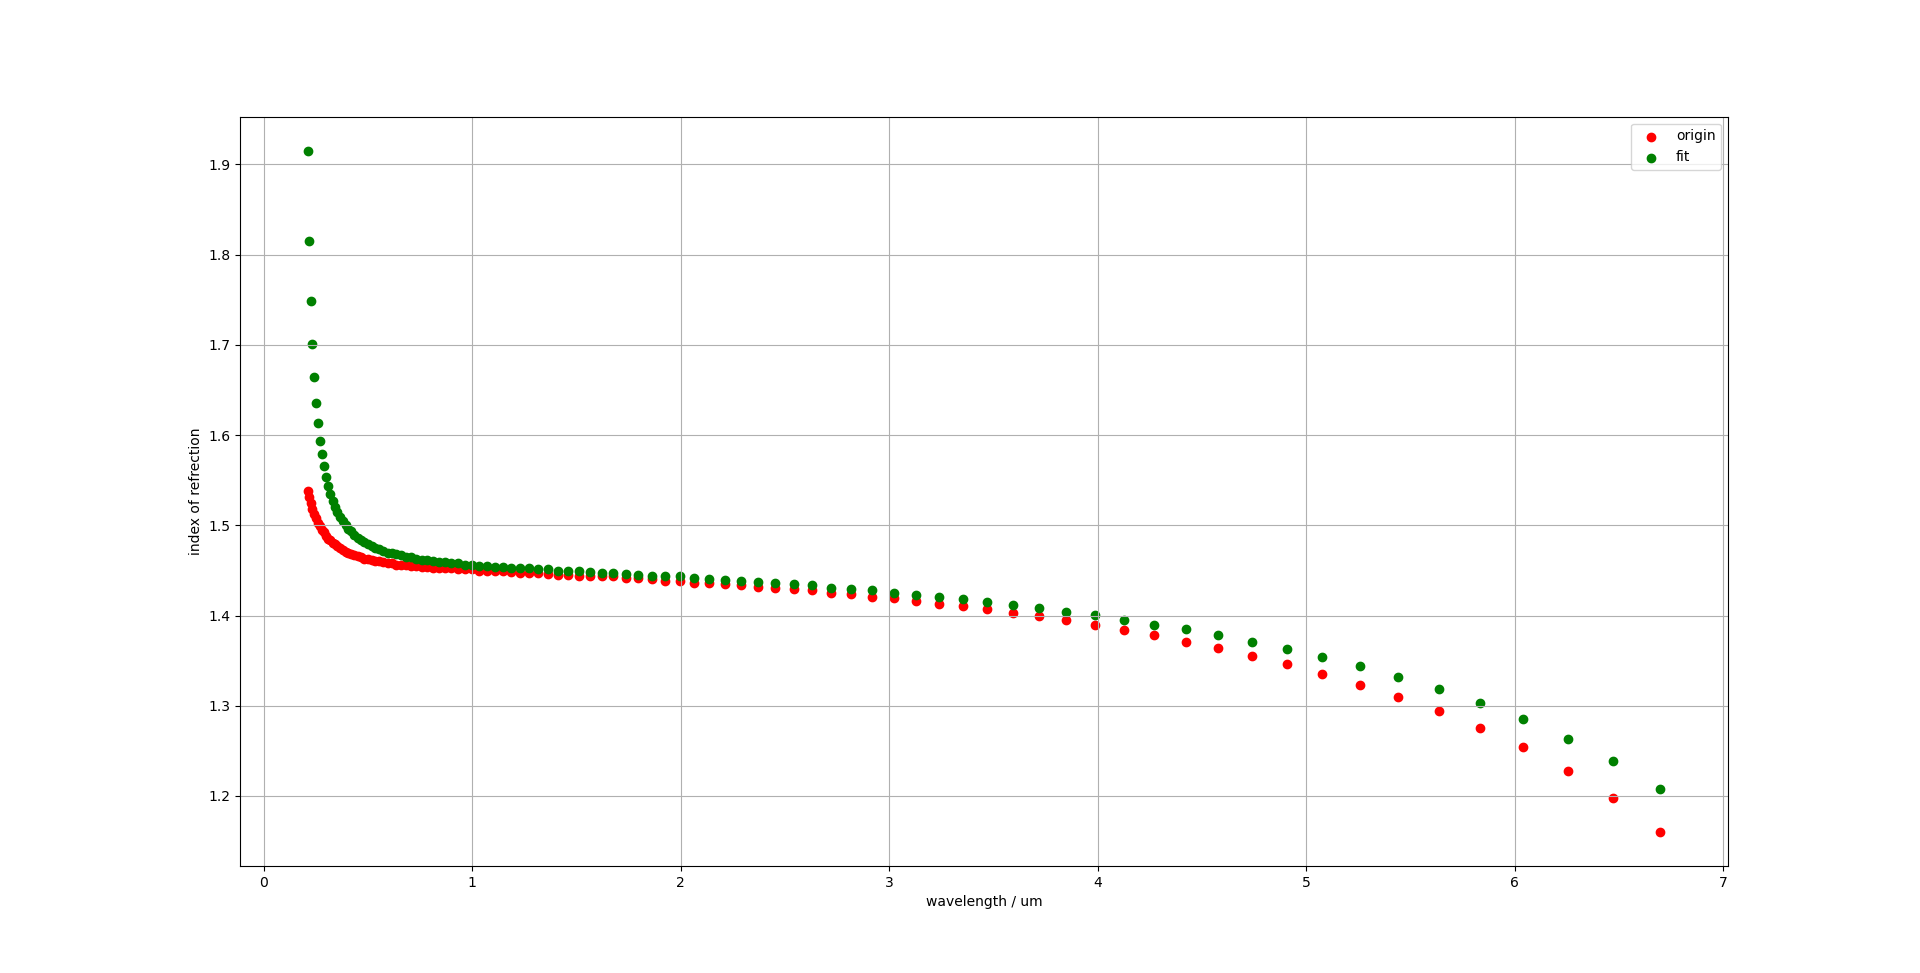
\includegraphics[width=15cm,height=9cm]{OandF.png}
    \caption{原始以及拟合后Sellmeir公式曲线对比}
\end{figure}

\end{document}
